\chapter{IMPLEMENTASI}
Setelah melewati proses perancangan mengenai sistem yang akan dibuat, maka akan dilakukan implementasi dari sistem tersebut. Bab ini akan membahas mengenai implementasi dari sistem yang meliputi proses pembuatan setiap komponen sehingga sistem dapat berjalan dengan baik. Masing-masing proses pembuat komponen akan dilengkapi dengan \textit{pseudocode} atau konfigurasi dari sistem.  
\section{Lingkungan Implementasi}
Dalam mengimplementasikan sistem, digunakan beberapa perangkat pendukung sebagai berikut.
\subsection{Perangkat Keras}
Perangkat keras yang digunakan dalam pengembangan sistem adalah sebagai berikut:
\begin{enumerate}
	\item Komputer dengan \textit{processor} Intel(R) Core(TM) i5-2120 CPU @ 3.30GHz dan RAM 8GB
	\item Komputer dengan \textit{processor} Intel(R) Core(TM)2 Duo CPU E7200 @ 2.53GHz dan RAM 1GB
\end{enumerate}
\subsection{Perangkat Lunak}
Perangkat lunak yang digunakan dalam pengembangan sistem adalah sebagai berikut:
\begin{enumerate}
	\item Sistem Operasi Linux Mint 18.03 64 Bit sebagai \textit{docker host}.
	\item Sistem Operasi Ubuntu 16.04 LTS 64 Bit sebagai \textit{client}.
	\item Sistem Operasi Debian 8.6.0 64 Bit sebagai \textit{server login}.
	\item Python versi 2.7.12 untuk pengembangan web service. 
	\item Flask versi 1.0.2 sebagai kerangka kerja Python.0
	\item Nginx versi 1.10.3
	\item Mitmrproxy versi 3.0.4 untuk mencatat semua \textit{traffic} dari \textit{client}.
	\item MySQL versi 5.7.18 untuk Sistem Manajemen Basis Data.
	\item Docker versi 1.13.1 sebagai kontainer yang akan di pasangkan pada \textit{server}.
	\item Iptables versi 1.6.0 untuk membuat aturan terhadap \textit{client}.
\end{enumerate}

\section{Implementasi Pembuatan Halaman \textit{Login} dari Sebuah Sistem}
Halaman \textit{login} dibangun pada sebuah \textit{server} dengan IP \texttt{10.151.36.171}. Pada implementasi pembuatan halaman \textit{login} dari sebuah sistem menggunakan perangkat lunak antara lain:
\begin{enumerate}
	\item Python versi 3.5.2.
	\item Flask versi 1.0.2.
\end{enumerate}

Lalu sistem operasi yang digunakan adalah sistem operasi Debian 8.6.0 64 Bit, yang akan dipasang pada \textit{virtual machine} dengan menggunakan VirtualBox. Python akan berfungsi sebagai komponen dasar pembangunan sistem yang akan dibangun dengan menggunakan kerangka kerja Flask dengan IP \texttt{10.151.36.171} dan \textit{port} 4000. Implementasi pembuatan halaman \textit{login} dari sebuah sistem akan terbagi menjadi implementasi \textit{web service} dan implementasi basis data.

\subsection{Implementasi \textit{Web Service} pada Halaman \textit{Login}}
Diperlukan beberapa tahap, antara lain pemasangan perangkat lunak dan tahap konfigurasi. Tahap pemasangan perangkat lunak dan tahap konfigurasi pada \textit{server} untuk halaman \textit{login} dijelaskan pada Lampiran A. 

Pada sub-bab implementasi \textit{web service} pada halaman \textit{login} akan dibagi lagi menjadi tiga bagian, antara lain implementasi tampilan antarmuka halaman \textit{login}, rute \textit{web service} pada halaman \textit{login} dan \textit{pseduocode web service} pada halaman \textit{login}.

\subsubsection{Implementasi Tampilan Antarmuka Halaman \textit{Login}}
Halaman \textit{login} merupakan halaman utama yang menampilkan sebuah \textit{form input} untuk \textit{client}. Pada halaman ini terdapat dua \textit{form input}, yaitu \textit{form input} untuk \texttt{Username} atau NRP dari \textit{client} dan juga \textit{form input} untuk \texttt{Password} dari \textit{client}. Implementasi antarmuka halaman \textit{login} dapat dilihat pada Gambar \ref{implementasihalamanlogin}.

\begin{figure}[H]
	\centering
	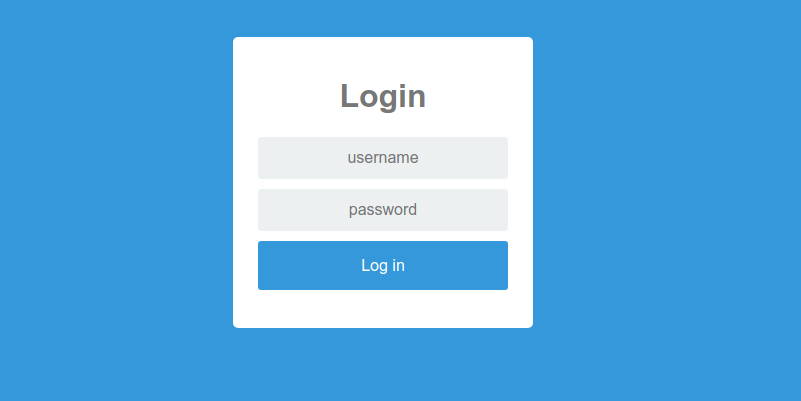
\includegraphics[width=10cm,height=5cm]{images/bab4/halamanlogin}
	\caption{Halaman \textit{Login}}
	\label{implementasihalamanlogin}
\end{figure}

\subsubsection{Rute \textit{Web Service} pada Halaman \textit{Login}}
Pada halaman \textit{login} diperlukan adanya rute-rute yang bisa diakses untuk melayani \textit{client}, supaya \textit{client} dapat membuka tampilan antar muka dari halaman \textit{login} dan juga supaya \textit{client} dapat mengirimkan permintaan untuk membuat kontainer \textit{docker} pada \textit{docker host}. Daftar rute yang disediakan oleh halaman \textit{loign} tertera pada Tabel \ref{tabelRuteWebServiceHalamnLogin}.\\
\begin{longtable}{|p{0.15\textwidth}|p{0.25\textwidth}|p{0.4\textwidth}|p{0.3\textwidth}|} % L = Rata kiri untuk setiap kolom, | = garis batas vertikal.
	
	% Kepala tabel, berulang di setiap halaman
	\caption{Daftar Rute \textit{Web Service}} \label{tabelRuteWebServiceHalamnLogin} \\
	\hline
	\textbf{HTTP Method} & \textbf{Rute} & \textbf{Deskripsi} \\ \hline
	
	\endfirsthead
	\caption[]{Daftar Rute \textit{Web Service}}  \\
	\hline
	\textbf{HTTP Method} & \textbf{Rute} & \textbf{Deskripsi}  \\ \hline
	
	\endhead
	\endfoot
	\endlastfoot
	
	% Isi Tabel
	GET & / & Berfungsi untuk mengarahkan \textit{redirect} ke rute \textit{login} dengan \textit{method} GET.\\ \hline
	GET & /login & Berfungsi untuk menampilkan tampilan grafis antar muka halaman \textit{login} ketika \textit{client} belum \textit{login} ke dalam sistem dan untuk menampilkan tampilan grafis antar muka halaman sukses \textit{login} ketika \textit{client} telah berasil \textit{login} ke dalam sistem.\\ \hline
	POST & /login & Berfungsi untuk menyimpan data hasil \textit{input} dari \textit{client} dan mengirimkan perintah untuk membuat kontainer \textit{docker} yang berisikan Mitmproxy secara otomatis pada \textit{docker host}.\\ \hline
	GET & /logout & Berfungsi untuk keluar dari sistem dan kontainer \textit{docker} yang sudah dibuat untuk \textit{client} yang telah berhasil \textit{login} dengan menggunakan \textit{username} tersebut akan di-\textit{destroy}. Lalu aturan-aturan yang sudah dibuat dengan menggunakan Iptables untuk \textit{client} tersebut juga dihapuskan.\\ \hline
	
\end{longtable}

\subsubsection{\textit{Pseduocode Web Service} pada Halaman \textit{Login}}
Ketika \textit{client} belum \textit{login} ke dalam sistem, maka akan diarahkan ke tampilan grafis antar muka dari halaman \textit{login}. Lalu setelah \textit{client} berhasil \textit{login} ke dalam sistem, maka akan diarahkan ke tampilan grafis antar muka halaman sukses \textit{login}. Pada Kode Sumber \ref{pseudocodehalamanlogin} diperlihatkan bagaimana implementasinya dalam bentuk \textit{pseduocode}.
\newline
\newline
\newline
\newline
\newline
\newline
\newline
\newline
\newline

\begin{minipage}{\linewidth}  
	\begin{lstlisting}[numbers=left, frame=single,tabsize=2,breaklines,caption={Pseudocode Web Service},label=pseudocodehalamanlogin,language=json]
	Check whether the client is already login or not yet
	
	if session.get login
		open welcome page
		
	else
		open login page
		
		if login success
			session.get login = True
			send request to docker host
	
	return  	
	\end{lstlisting}
\end{minipage}


\subsection{Implementasi Basis Data pada Halaman \textit{Login}}
Berdasarkan hasil desain dan perancangan basis data pada bab 3 terdapat satu entitas yang diimplementasikan menjadi suatu tabel pada basis data MySQL, yaitu entitas \texttt{nrp-mahasiswa}. Detail implementasi \textit{query} untuk membuat basis data dengan entitas \texttt{nrp-mahasiswa} seperti pada Gambar \ref{querynrpmahasiswa}.\\
\begin{figure}[H]
	\centering
	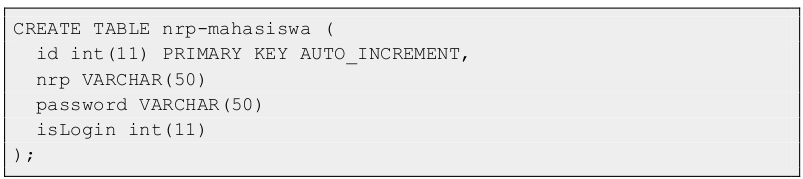
\includegraphics[width=\linewidth]{images/bab4/querynrpmahasiswa}
	\caption{\textit{Query} untuk membuat tabel kontainer}
	\label{querynrpmahasiswa}
\end{figure}


\section{Implementasi Pembuatan Aturan untuk Mengarahkan \textit{Traffic Client} ke Halaman \textit{Login} dari Sistem}
Pada implementasi pembuatan aturan untuk mengarahkan \textit{traffic client} ke halaman \textit{login} dari sistem diasumsikan bahwa belum ada \textit{client} yang telah \textit{login} ke dalam sistem. Karena diasumsikan bahwa belum ada \textit{client} yang telah berhasil \textit{login} ke dalam sistem, maka semua \textit{client} tidak diperbolehkan untuk mengakses internet. Kemudian untuk mengarahkan \textit{traffic} dari \textit{client} dibuatkan beberapa \textit{rules} dengan menggunakan iptables pada \textit{Docker Host} dengan IP \texttt{10.151.36.134}. seperti Gambar \ref{iptablesbeforelogin}.
\begin{figure}[H]
	\centering
	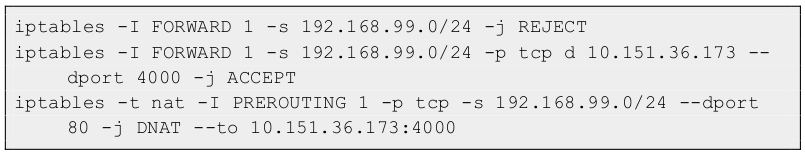
\includegraphics[width=\linewidth]{images/bab4/iptables1}
	\caption{Command untuk mengarahkan \textit{client} ke halaman \textit{login}}
	\label{iptablesbeforelogin}
\end{figure}

\indent \textit{Rules} pertama berfungsi untuk melarang semua \textit{client} untuk melewati \textit{router}. \textit{Rules} kedua berfungsi untuk mengizinkan semua \textit{client} membuka halaman \textit{login}. Sedangkan \textit{rules} ketiga berfungsi untuk mengarahkan semua \textit{traffic client} ke halaman \textit{login}.

\section{Implementasi Pembuatan \textit{Middleware}}
\textit{Middleware} dibangun pada \textit{Docker Host} dengan IP \texttt{10.151.36.134} dengan menggunakan sistem operasi Linux Mint 18.03 64 Bit. \textit{Middleware} merupakan komponen yang akan menerima permintaan dari \textit{client}, mengirimkan perintah untuk membuat kontainer \textit{docker} secara otomatis pada \textit{docker host}, dan menentukan rute \textit{traffic} dari \textit{client} menuju ke internet sesuai kontainer \textit{docker} masing-masing user. Implementasi \textit{middleware} akan terbagi menjadi implementasi basis data dan implementasi \textit{web service}.

Pada implementasi pembuatan \textit{middleware} menggunakan perangkat unak antara lain:
\begin{enumerate}
	\item Python versi 2.7.12.
	\item Flask versi 1.0.2.
	\item Docker versi 1.13.1.
\end{enumerate}

Python akan berfungsi sebagai komponen dasar pembangunan sistem, salah satunya adalah sebagai komponen dasar pembuatan \textit{middleware}, sedangkan Flask akan berfungsi sebagai kerangka kerja untuk pembuatan \textit{middleware}. Implementasi pembuatan \textit{middleware} akan terbagi menjadi implementasi \textit{web service} dan implementasi basis data dan.

\subsection{Implementasi \textit{Web Service} pada \textit{Middleware}}
Diperlukan beberapa tahap, antara lain pemasangan perangkat lunak dan tahap konfigurasi. Tahap pemasangan perangkat lunak dan tahap konfigurasi pada \textit{middleware} di \textit{Docker Host} dijelaskan pada Lampiran A.

Pada sub-bab implementasi \textit{web service} pada \textit{middleware} akan dibagi lagi menjadi dua bagian, antara lain rute \textit{web service} pada \textit{middleware} dan juga \textit{pseduocode web service} pada \textit{middleware}.

\subsubsection{Rute \textit{Web Service} pada \textit{Middleware}}
\textit{Middleware} tidak memiliki antar muka grafis. Namun tetap diperlukan adanya rute-rute yang bisa diakses untuk melayani permintaan penyediaan kontainer \textit{docker} dari \textit{client}. Daftar rute yang disediakan oleh \textit{middleware} tertera pada Tabel \ref{tabelRuteWebServiceDockerHost}.\\
\begin{longtable}{|p{0.15\textwidth}|p{0.25\textwidth}|p{0.4\textwidth}|p{0.3\textwidth}|} % L = Rata kiri untuk setiap kolom, | = garis batas vertikal.
	
	% Kepala tabel, berulang di setiap halaman
	\caption{Daftar Rute \textit{Web Service}} \label{tabelRuteWebServiceDockerHost} \\
	\hline
	\textbf{HTTP Method} & \textbf{Rute} & \textbf{Deskripsi} \\ \hline
	
	\endfirsthead
	\caption[]{Daftar Rute \textit{Web Service}}  \\
	\hline
	\textbf{HTTP Method} & \textbf{Rute} & \textbf{Deskripsi}  \\ \hline
	
	\endhead
	\endfoot
	\endlastfoot
	
	% Isi Tabel
	POST & /test/endpoint/ & Berfungsi untuk menyimpan data hasil \textit{input} dari \textit{client} dan mengirimkan perintah untuk membuat kontainer \textit{docker} yang berisikan \textit{mitmproxy} secara otomatis pada \textit{docker host}.\\ \hline
	POST & /logout/endpoint/ & Berfungsi untuk menerima permintaan penghentian akses internet dari \textit{client} sendiri dan juga untuk menjalankan perintah penghapusan kontainer \textit{docker} dan \textit{rules} dari \textit{client} tersebut. Setelah pada basis data \texttt{kontainer} akan dilakukan pembaruan \textit{status} dari kontainer yang telah digunakan oleh \textit{client} tersebut menjadi 0.\\ \hline
\end{longtable}

\subsubsection{\textit{Pseduocode Web Service} pada \textit{Middleware}}
Saat \textit{client} telah memasukkan \textit{input} ke sistem, sistem akan mencocokkan terlebih dahulu dengan basis data \texttt{kontainer}. Jika benar, maka sistem akan mengirimkan data \textit{input} dari \textit{client} ke \textit{middleware}. Lalu \textit{middleware} akan menyimpan data \textit{input} dari \textit{client} ke dalam sebuah \textit{file}. Setelah itu \textit{middleware} akan mengirimkan perintah untuk membuat sebuah kontainer \textit{docker} yang berisikan Mitmproxy pada \textit{docker host}.

Saat \textit{middleware} menyimpan data \textit{input} dari \textit{client} ke dalam sebuah \textit{file}, yang disimpan adalah \textit{username} atau NRP, \textit{IP Address}, dan \textit{port}. Nantinya \textit{port} tersebut akan menjadi \textit{port} khusus untuk kontainer \textit{docker} yang berisikan \textit{mitmproxy} untuk \textit{client} tersebut.

Saat kontainer \textit{docker} yang berisikan \textit{mitmproxy} akan dibuat pada \textit{docker host}, sistem akan membuat kontainer \textit{docker} dengan \textit{mode network}=\textit{host}, nama sesuai \textit{IP Address} dari \textit{client} tersebut, dan \textit{port} kontainer \textit{docker} sesuai dengan \textit{port} yang sudah disimpan pada \textit{file}.

Setelah kontainer \textit{docker} yang berisikan \textit{mitmproxy} berhasil dibuat, maka sistem akan membuat \textit{rules} yang berfungsi untuk mengarahkan \textit{traffic} dari \textit{client} menuju ke kontainer \textit{docker} milik \textit{client} tersebut, dan memperbolehkan \textit{client} untuk mengakses internet. Pada Kode Sumber \ref{pseudocodeoing} diperlihatkan bagaimana implementasinya dalam bentuk \textit{pseduocode}.
\newline

\begin{minipage}{\linewidth}  
	\begin{lstlisting}[numbers=left, frame=single,tabsize=2,breaklines,caption={Pseudocode Web Service},label=pseudocodeoing,language=json]
	Check whether the client is already login or not yet
	
	if session.get login
		create container
		add new rules to container
	
	else
		add new rules to page login
	
	return  	
	\end{lstlisting}
\end{minipage}

\subsection{Implementasi Basis Data pada \textit{Middleware}}
Berdasarkan hasil perancangan basis data pada bab 3 terdapat 2 entitas yang diimplementasikan menjadi suatu tabel pada basis data MySQL, yaitu entitas \texttt{kontainer}. Detail implementasi entitas \texttt{kontainer} tertera pada Gambar \ref{querykontainer}.


\section{Implementasi Pemasangan Kontainer Docker pada \textit{Docker Host}}
Setelah berhasil melakukan pemasangan \textit{docker} versi 1.13.1 pada \textit{docker host} dengan IP \texttt{10.151.36.134}, sekarang lakukan konfigurasi supaya \textit{docker} tidak hanya dapat digunakan oleh \textit{root user} dari sebuah sistem. Hal ini dapat dilakukan dengan menjalankan perintah pada Gambar \ref{konfigurasildocker1}.
\begin{figure}[H]
	\centering
	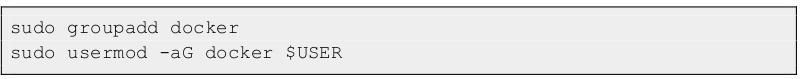
\includegraphics[width=\linewidth]{images/bab4/konfigurasildocker1}
	\caption{Perintah memasukkan \textit{user} ke grup \textit{docker}}
	\label{konfigurasildocker1}
\end{figure}


\subsection{Menambahkan dan Memperbarui Kontainer Docker yang Berisikan Mitmproxy}
Setelah berhasil melakukan pemasangan \textit{docker} pada \textit{docker host} dan melakukan konfigurasi supaya \textit{docker} tidak hanya dapat digunakan oleh \textit{root user} dari sebuah sistem, selanjutnya dapat mencoba membuat sebuah kontainer \textit{docker} yang berisi aplikasi Mitmproxy. Untuk membuat sebuah kontainer \textit{docker} yang berisi Mitmproxy, penulis melakukannya dengan sistem operasi Ubuntu dalam format \textit{docker} yang disediakan oleh \textit{Docker Hub}. Untuk melakukan unduh, jalankan perintah \texttt{docker pull ubuntu}.

Setelah berhasil diunduh, selanjutnya jalankan sistem operasi Ubuntu dengan menggunakan perintah \texttt{docker run --name testmitmproxy --privileged=True --network=host ubuntu}.

Parameter \texttt{--name} berguna untuk memberikan nama pada kontainer \textit{docker} agar mudah dikenali dimana lokasi aplikasi saat dijalankan. Pada kasus ini kontainer \textit{docker} diberi nama dengan \texttt{testmitmproxy}. Parameter \texttt{--privileged=True} berguna untuk memberikan kendali hak akses penuh kepada kontainer \textit{docker} tersebut, sama seperti dengan \textit{root user}. Parameter \texttt{--network=host} berguna untuk mendefinisikan jaringan yang akan digunakan oleh kontainer \textit{docker} tersebut. Setelah menjalankannya, kontainer \textit{docker} yang terbentuk dapat digunakan lebih lanjut, misalnya dengan mengubah data yang ada didalamnya, menambahkan fitur baru, atau hanya sekedar mengganti nama dari aplikasi.\\
\indent Dalam kasus ini penulis menambahkan fitur baru, yaitu menambah Mitmproxy. Untuk menambah atau memasang Mitmproxy pada kontainer \textit{docker} yang baru saja dibuat, jalankan perintah berikut pada Gambar \ref{installmitmproxy}.

\begin{figure}[H]
	\centering
	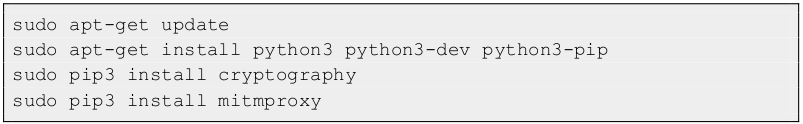
\includegraphics[width=\linewidth]{images/bab4/installmitmproxy}
	\caption{Perintah untuk Pemasangan Mitmrproxy}
	\label{installmitmproxy}
\end{figure}

Mitmrproxy versi 3.0.4 membutuhkan Python minimal versi 3.5, maka dari itu penulis memasang Python versi 3.5.2. Mitmrproxy juga membutuhkan modul \textit{cryptography} yang berguna untuk melakukan enkripsi maupun dekripsi ketika Mitmproxy sedang berjalan. Lalu aktifkan \texttt{ipv4.forwarding} dengan menjalankan perintah \texttt{sudo sysctl -w net.ipv4.ip-forward=1}.

Setelah berhasil melakukan pemasangan Mitmproxy pada kontainer \textit{docker}, jika ingin membuat \textit{images} baru dari kontainer \textit{docker} tersebut, maka hal pertama yang harus dilakukan adalah menghentikan kontainer \textit{docker} yang sedang berjalan dengan menggunakan perintah \texttt{docker stop [nama container]}.

Nama \textit{container} ini tergantung dari nama kontainer \textit{docker} yang sudah dibuat. Untuk kasus yang digunakan oleh penulis, penulis menggunakan perintah \texttt{docker stop testmitmproxy}. Setelah itu lakukan \textit{commit} dengan menjalankan perintah \texttt{docker commit [nama container] [nama repository]}.

Nama \textit{container} ini tergantung dari nama kontainer \textit{docker} yang sudah dibuat. Sedangkan nama \textit{repository} ini tergantung dari nama \textit{repository} yang telah dibuat di Docker Hub. Untuk kasus yang digunakan oleh penulis, penulis menggunakan perintah \texttt{docker commit testmitmproxy fourirakbar/mitmproxy-oing:version1}. Pada bagian nama \textit{repository} ini memiliki tiga bagian dengan pola seperti \texttt{[URL]/[nama]:[versi]}. Artinya membuat \textit{image} dengan URL \textit{repository} pada Docker Hub dengan nama \texttt{fourirakbar}. Kemudian nama dari \textit{image}-nya sendiri adalah \texttt{mitmproxy-oing} dan versinya adalah \texttt{version1}. Setelah melakukan \textit{commit}, maka \textit{image} baru akan terbentuk. Langkah terakhir adalah melakukan \textit{push image} ke Docker Hub dengan menggunakan perintah \texttt{docker push [nama container] [nama repository]}.

\subsection{Menggunakan \textit{Image} Kontainer Docker yang Sudah Dibuat}
Setelah berhasil menambahkan dan memperbarui kontainer \textit{docker} yang berisi Mitmproxy, penulis tidak perlu melakukannya lagi. Penulis hanya perlu memanggil kontainer \textit{docker} dengan menjalankan perintah \texttt{docker pull fourirakbar/mitmproxy-oing:version1}.

Lalu untuk menjalankan kontainer \textit{docker} yang sudah di \textit{pull}, jalankan perintah \texttt{docker run --name [IP CLEINT] --privileged=True --network=host fourirakbar/mitmproxy-oing:version1}.

\section{Implementasi Pembuatan Aturan untuk Mengarahkan \textit{Traffic Client} ke Kontainer Docker dari Tiap-Tiap \textit{Client}}
Pada implementasi pembuatan aturan untuk mengarahkan \textit{traffic client} ke kontainer \textit{docker} dari tiap-tiap client dibuat ketika terdapat \textit{client} yang telah berhasil \textit{login} ke dalam sistem. Setelah \textit{client} berhasil \textit{login} ke dalam sistem, maka akan dibuatkan beberapa \textit{rules} dengan menggunakan Iptables seperti Gambar \ref{iptablesafterlogin}.
\begin{figure}[H]
	\centering
	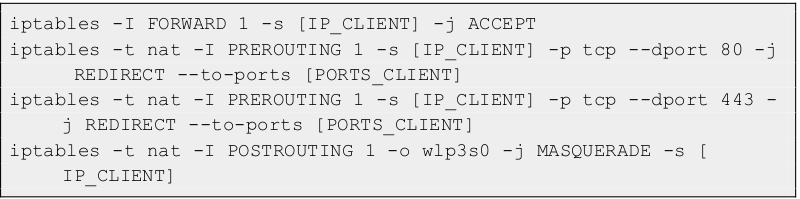
\includegraphics[width=\linewidth]{images/bab4/iptablesafterlogin}
	\caption{Command untuk mengarahkan \textit{client} ke halaman \textit{login}}
	\label{iptablesafterlogin}
\end{figure}

Pada \textit{rules} pertama berfungsi untuk mengizinkan atau memperbolehkan \textit{traffic} dari \textit{client} melewati \textit{router}. Lalu \textit{rules} kedua dan ketiga berfungsi untuk mengarahkan \textit{traffic cleint} ke kontainer \textit{docker} yang sudah dibuat dengan satu port khusus untuk \textit{client} tersebut. Lalu \textit{rules} keempat berfungsi untuk mengizinkan atau memperbolehkan \textit{client} untuk mengakses internet.

\section{Implementasi Pembuatan Halaman \textit{Administrator}}
Halaman \textit{administrator} dibangun pada \textit{Docker Host} dengan IP \texttt{10.151.36.134} dengan port \texttt{5001}. Fungsi dari halaman \textit{administrator} adalah untuk melihat siapa saja \textit{client} yang berhasil \textit{login} ke dalam sistem dan megnakses internet, juga untuk melihat rekap \textit{client} yang telah berhasil \textit{login} dan mengakses internet. Selain itu juga dapat menghentikan akses penggunaan internet dari \textit{client}. Pada sub-bab ini akan dibagi lagi menjadi beberapa bagian, antara lain rute \textit{web service} pada halaman \textit{administrator}, implementasi pembacaan \textit{log file} dari \textit{client} dan implementasi antarmuka.

\subsection{Rute \textit{Web Service} pada Halaman \textit{Administrator}}
Pada halaman \textit{administrator} diperlukan adanya rute-rute yang bisa diakses untuk melayani permintaan dari \textit{user} yang sedang membuka hallaman \textit{administrator}, yaitu untuk melihat \textit{log} dari \textit{client}. Daftar rute yang disediakan tertera pada Tabel \ref{rutehalamanadmin}.\\
\begin{longtable}{|p{0.1\textwidth}|p{0.2\textwidth}|p{0.25\textwidth}|p{0.3\textwidth}|} % L = Rata kiri untuk setiap kolom, | = garis batas vertikal.
	
	% Kepala tabel, berulang di setiap halaman
	\caption{Daftar Rute \textit{Web Service} pada Halaman \textit{Administrator}} \label{rutehalamanadmin} \\
	\hline
	\textbf{HTTP Method} & \textbf{Rute} & \textbf{Parameter} & \textbf{Deskripsi} \\ \hline
	
	\endfirsthead
	\caption[]{Daftar Rute \textit{Web Service}}  \\
	\hline
	\textbf{HTTP Method} & \textbf{Rute} & \textbf{Parameter} & \textbf{Deskripsi}  \\ \hline
	
	\endhead
	\endfoot
	\endlastfoot
	
	% Isi Tabel
	GET & /table & - & Berfungsi untuk menampilkan halaman \textit{dashboard} yang menunjukkan siapa saja \textit{client} yang telah berhasil \textit{login} ke dalam sistem dan sedang aktif mengakses internet.\\ \hline
	GET & /stream/ & \texttt{id, ip, user, port} & Berfungsi untuk melihat \textit{log} dari \textit{client} secara langsung atau \textit{live} dengan memasukkan parameter berupa \texttt{id}, \texttt{ip}, \texttt{user}, dan \texttt{port}.\\ \hline
	GET & /lihat/ & \texttt{id, ip, user, port} & Berfungsi untuk melihat \textit{log} dari \textit{client} sampai dengan terakhjir \textit{client} mengakses internet dengan memasukkan parameter berupa \texttt{id}, \texttt{ip}, \texttt{user}, dan \texttt{port}.\\ \hline
	GET & /history & - & Berfungsi untuk menampilkan rekap atau daftar \textit{client} yang telah berhasil \textit{login} ke dalam sistem.\\ \hline
	GET & /stop/ & \texttt{id, ip, user, port} & Berfungsi untuk menghentikan akses penggunaan internet dari sebuah \textit{client} dengan memasukkan parameter berupa \texttt{id}, \texttt{ip}, \texttt{user}, dan \texttt{port}.\\ \hline
\end{longtable}

\subsection{Implementasi Pembacaan \textit{Log File} dari \textit{Client}}
Pada implementasi pembacaan \textit{log file} dari \textit{client} dilakukan dengan membaca \textit{file} hasil \textit{output} dari \textit{mitmproxy}. \textit{File} hasil \textit{output} dari \textit{mitmproxy} berbentuk \textit{binary} dimana yang bisa membacanya hanya komputer saja. Maka dari itu perlu dilakukan pembacaan lagi \textit{file} yang berisi \textit{binary} tersebut dengan menjalankan \textit{command} \texttt{mitmdump -nr [NAMA-FILE] --set flow-detail=2 --showhost > [NAMA-FILE]}.

Sedangkan untuk membaca \textit{log file} dari \textit{client} secara langsung atau \textit{live} dapat dilakukan dengan menjalankan \textit{command} \texttt{tail -f -c +0 [NAMA FILE] | mitmdump -n -r - --set flow detail=1 --showhost}.

Parameter \texttt{-nr} berfungsi untuk tidak menjalankan \textit{proxy server} dari \textit{mitmproxy} sendiri, dan juga berfungsi untuk melakukan analisa dari \textit{file output mitmproxy} yang berbentuk \textit{binary}. Sedangkan parameter \texttt{--set flow detail} berfungsi untuk menampilkan detail dari analisa yang dilakukan oleh \textit{mitmproxy}. Terdapat tingkat satu sampai dengan tiga, semakin tinggi tingkat yang diberikan maka semakin jelas detail dari \textit{log} yang dianalisa oleh \textit{mitmproxy}. Lalu parameter \texttt{--showhost} berfungsi untuk menampilkan \textit{header} dari URL yang telah diakses oleh \textit{client}.

\subsection{Implementasi Antarmuka Halaman \textit{Administrator}}
Halaman \textit{administrator} diperuntukkan bagi \textit{User} yang mempunyai akses ke \textit{Docker Host}. Halaman ini berguna sebagai \textit{dashboard} dari \textit{administrator}. Pada halaman ini menampilkan siapa saja \textit{Client} yang telah berhasil \textit{login} ke dalam sistem. Terdapat dua \textit{button}, yaitu \textit{Stream Log} yang berfungsi untuk melihat secara langsung atau \textit{live log} dari \textit{client}. Lalu terdapat \textit{button} Lihat \textit{Log} yang berfungsi untuk melihat \textit{log} dari \textit{client} sampai terakhir \textit{client} tersebut mengakses internet.

\begin{figure}[H]
	\centering
	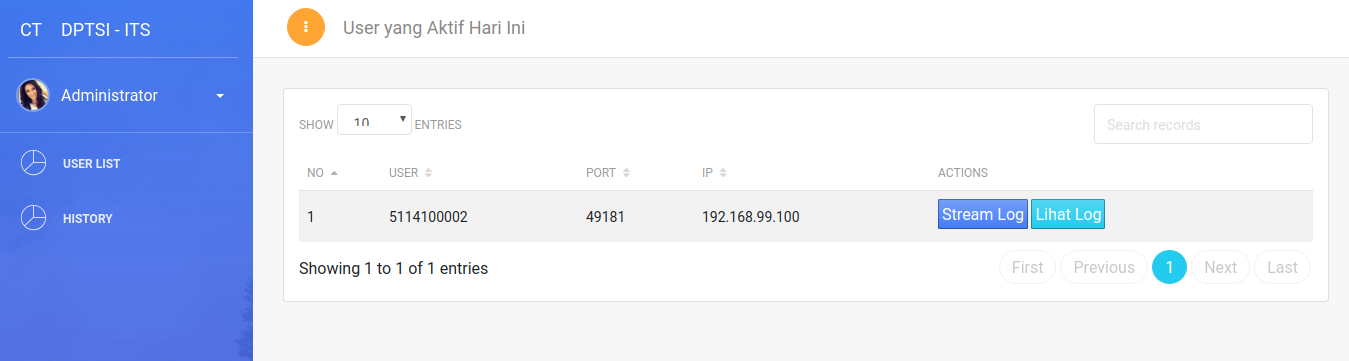
\includegraphics[width=\linewidth]{images/bab4/useraktif}
	\caption{Halaman \textit{Administrator} Menu \textit{User List}}
	\label{halamandashboardadmin}
\end{figure}

Pada bagian \textit{sidebar} terdapat dua menu yaitu \textit{User List} dan \textit{History}. Menu \textit{User List} berguna untuk melihat \textit{client} yang telah berhasil \textit{login} ke dalam sistem. Sedangkan menu \textit{history} berguna untuk melihat rekap \textit{client} yang telah berhasil \textit{login} dan mengakses internet pada hari-hari sebelumnya. Implementasi antarmuka halaman \textit{administrator} pada menu \textit{User List} dapat dilihat pada Gambar \ref{halamandashboardadmin}. Dan implementasi antarmuka halaman \textit{administrator} oada nenu \textit{History} dapat dilihat pada Gambar \ref{userrekap}
\newline
\newline
\newline

\begin{figure}[H]
	\centering
	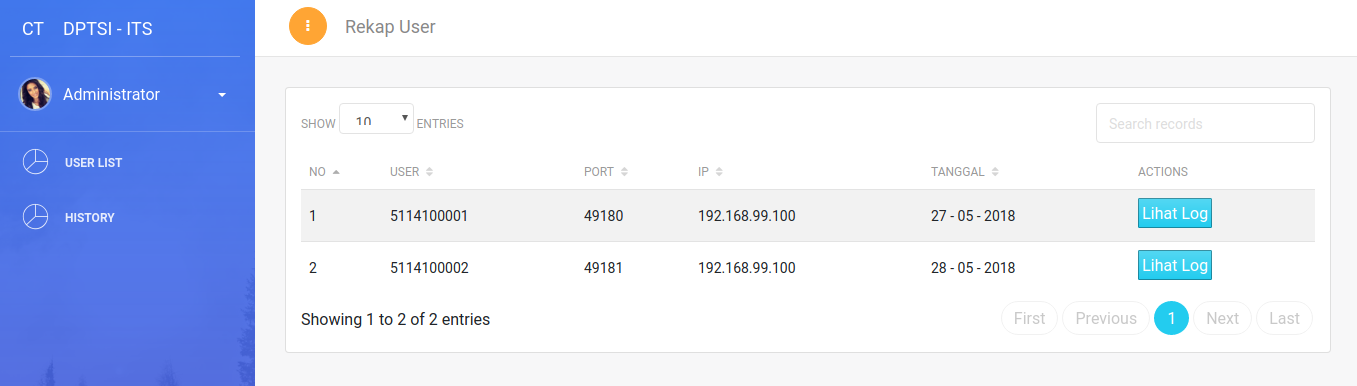
\includegraphics[width=\linewidth]{images/bab4/userrekap}
	\caption{Halaman \textit{Administrator} Menu \textit{History}}
	\label{userrekap}
\end{figure}